\documentclass[tikz,border=10pt]{standalone}
\usepackage{tikz}
\usetikzlibrary{calc}
\usetikzlibrary{positioning}
\usetikzlibrary{shapes}

\begin{document}
    \tikzstyle{every node}=[fill=white, draw=black, circle, minimum size=0.6cm]
    \tikzstyle{labelright}=[font=\scriptsize, xshift=0.5em, yshift=-1.5em, draw=none, fill=none]
    \tikzstyle{labelleft}=[font=\scriptsize, xshift=-0.5em, yshift=-1.5em, draw=none, fill=none]
    \tikzstyle{canoe}=[pos=0.15,fill=none,draw=none]
    \begin{tikzpicture}[auto, node distance=2cm, thick]
    \node (0) {0};
    \node [right of=0] (1) {1};
    \node [below of=1] (2) {2};
    \node [left  of=2] (3) {3};

    \draw (0) -- (1) node[canoe,yshift=-0.5em,label={[labelright]0}]{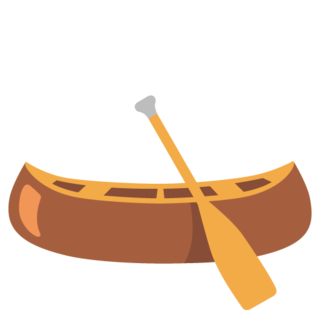
\includegraphics[width=1em]{canoe.png}};
    \draw (1) -- (2) node[canoe,xshift=-0.5em,label={[labelright]1}]{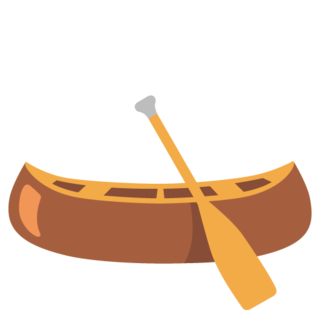
\includegraphics[width=1em,angle=270]{canoe.png}};
    \draw (2) -- (3) node[canoe,above,yshift=-0.5em,label={[labelleft]2}]{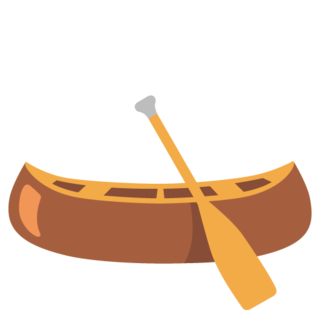
\includegraphics[width=1em]{canoe.png}};
    \draw (0) -- (3) node[canoe,left, xshift=+0.5em,label={[labelleft]3}]{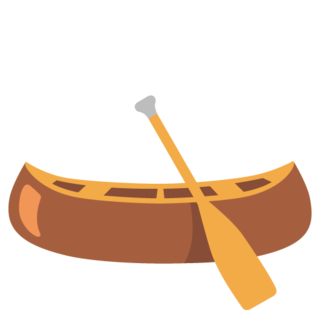
\includegraphics[width=1em,angle=90]{canoe.png}};
    \draw (3) -- (1) node[canoe,xshift=0.5em,yshift=-0.5em,label={[labelright]4}]{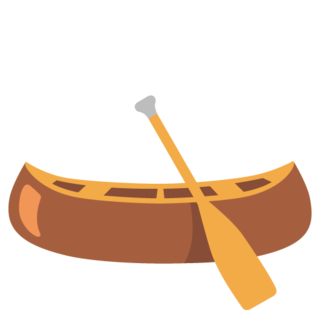
\includegraphics[width=1em,angle=45]{canoe.png}};
\end{tikzpicture}

    \begin{tikzpicture}[auto, node distance=2cm, thick]
    \node (0) {0};
    \node [right of=0] (1) {1};

    \draw (0) -- (1) node[canoe,yshift=-0.5em,label={[labelright]0}]{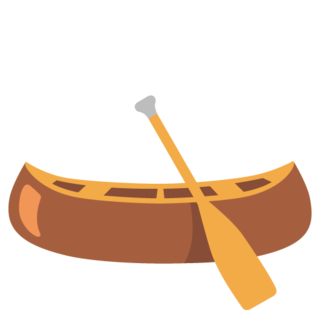
\includegraphics[width=1em]{canoe.png}};
    \draw (1) -- (0) node[canoe,above,yshift=-0.5em,label={[labelleft]1}]{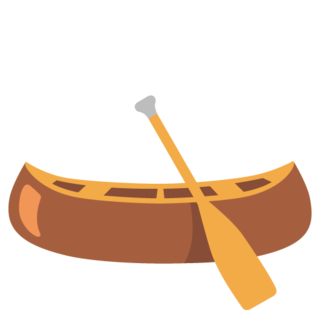
\includegraphics[width=1em]{canoe.png}};
    \draw (1) -- (0) node[canoe,below,yshift=+1.0em,label={[labelleft,below,yshift=0.3em]2}]{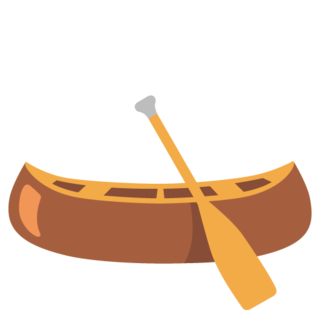
\includegraphics[width=1em]{canoe.png}};
\end{tikzpicture}

\end{document}
